\chapter{Results}
\label{sec:evaluation}

To evaluate the impact of removing permissions on applications, seven common permissions (Table~\ref{tbl:results}) were selected based on their potential threat to the user's security and privacy.  For each permission, 100 applications that declare the permission in their manifests were randomly downloaded.  These applications are from the official Google Play Market as well as other markets in the US, China, and Europe.

\begin{table*}[t]
\centering
\tiny
\begin{tabular}{|l|c|c|c|c|}
\hline
& \# Failed & \# Apps & \multicolumn{2}{|c|}{\texttt{SecurityException}} \\ \cline{4-5}
Data Set & APKTool & Run & \# Exceptions & \# Apps Throwing Exceptions\\ \hline 
{\bfseries \ttfamily WRITE\_SMS} Original & 0 & 99 & 0 & 0 \\ \hline
{\bfseries \ttfamily WRITE\_SMS} Removed & 0 & 99 & 0 & 0 \\ \hline
{\bfseries \ttfamily ACCESS\_FINE\_LOCATION} Original & 0 & 100 & 2 & 2 \\ \hline
{\bfseries \ttfamily ACCESS\_FINE\_LOCATION} Removed & 1 & 99 & 21 & 12 \\ \hline					
{\bfseries \ttfamily CAMERA} Original & 1 & 99 & 0 & 0 \\ \hline
{\bfseries \ttfamily CAMERA} Removed & 2 & 98 & 0 & 0 \\ \hline
{\bfseries \ttfamily RECORD\_AUDIO} Original & 0 & 100 & 0 & 0 \\ \hline
{\bfseries \ttfamily RECORD\_AUDIO} Removed & 4 & 96 & 0 & 0 \\ \hline
{\bfseries \ttfamily READ\_CALENDAR} Original & 0 & 99 & 0 & 0 \\ \hline 
{\bfseries \ttfamily READ\_CALENDAR} Removed & 0 & 99 & 19 & 6 \\ \hline
{\bfseries \ttfamily READ\_CONTACTS} Original & 1 & 99 & 0 & 0 \\ \hline
{\bfseries \ttfamily READ\_CONTACTS} Removed & 3 & 97 & 81 & 18 \\ \hline
{\bfseries \ttfamily INTERNET} Original & 0 & 99 & 84 & 3 \\ \hline
{\bfseries \ttfamily INTERNET} Removed & 0 & 99 & 84 & 3 \\ \hline
\end{tabular}
\caption{Results of Random UI Introspection}
\label{tbl:results}
\end{table*}


A small portion (less than 2\%) of the applications contained manifests with unusual control characters that APKTool would not process (eg. 0x04), and were discarded.  Additionally, a couple of the applications failed installation and consequently were not tested. \toolname\ installed and tested the remaining ones as described in Chapter~\ref{sec:methodology}. 

\toolname\ detects application crashes and their causes from the emulator's ActivityManager.  When an application does not have a permission required by an API call, the Android framework will typically throw a \texttt{SecurityException} and, unless it catches the exception, the application will crash.   For example, this occurs if there are bugs in the application, or when \toolname\ executes an activity that is not meant to be executed by the user.  An additional possibility is that a library acting on the application's behalf receives the \texttt{SecurityException} and returns the improper error condition.  Applications that do not check for this kind of error state may crash with other types of exceptions such as \texttt{NullPointerException}.  To identify errors caused by permission removal that are not \texttt{SecurityExceptions}, all the exceptions are tracked and plotted as you will see below.  Ultimately, since it is not possible to determine the true causes of these exceptions without extensive static analysis of each application, this study focuses on \texttt{SecurityExceptions}, which indicate under-permission.  The seven permissions and their application crash patterns are examined separately below.

%Among all the crashes, 5.8\% were due to a \texttt{SecurityException}.
%getaddrinfo failed: EACCES (Permission denied)

\paragraph{\bfseries \ttfamily INTERNET}
From a thorough examination of the logs, it was ascertained that the \texttt{SecurityExceptions} generated both before and after permission removal were the result of a change in the permissions system in Android 4.2.  For the API calls the applications performed, Android 4.2 requires a new permission, \texttt{WRITE\_APN\_SETTINGS}.  This is technically under-permission, but was not caused by removing existing permissions.  Analyzing the exceptions outside of \texttt{SecurityExceptions} resulted in the identification of the use of the Mobclix ad library, which requires the \texttt{INTERNET} permission~\cite{mobclix} and throws its own exception when it is removed, \texttt{com.mobclix.android.sdk.Mobclix\$MobclixPermissionException}, as well as 17 applications throwing \texttt{libcore.io.ErrnoException}.  From manual investigation of the stack dumps, the Mobclix exceptions were a result of removing the \texttt{INTERNET} permission and the \texttt{libcore.io.ErrnoException} instances were a result of a failed \texttt{getaddrinfo} request resulting from the removal of the \texttt{INTERNET} permission.  The \texttt{com.google.ads.AdActivity}.  For the remainder of the sample set, ad libraries were the sole reason for an application's request for the \texttt{INTERNET} permission.  All the versions of the \textit{AdMob} libraries that were examined fail gracefully when the INTERNET permission was removed.  For example,  one version of \textit{AdMob} displays a message to the user as seen in Figure~\ref{fig:removing}.    

com.google.ads.AdActivity   

%\FloatBarrier
\begin{figure}[h!]
\hfill
\subfigure[]{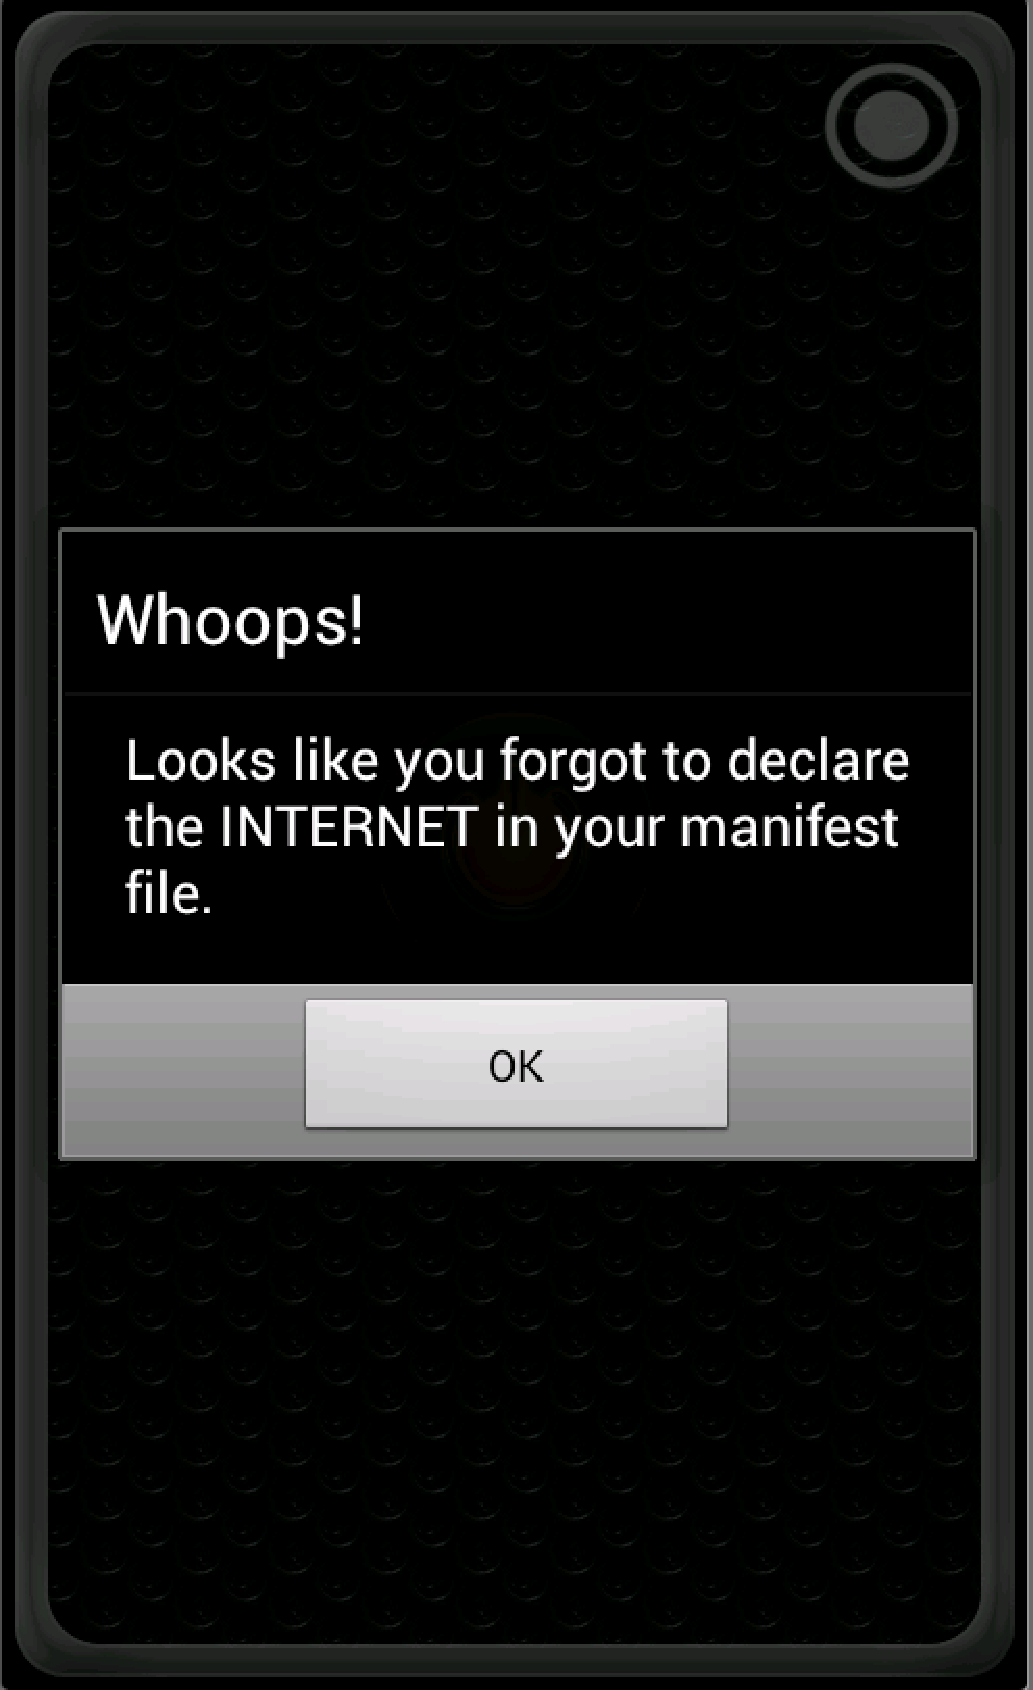
\includegraphics[scale=0.3]{figure2}\label{fig:removing}}
\hfill
\subfigure[]{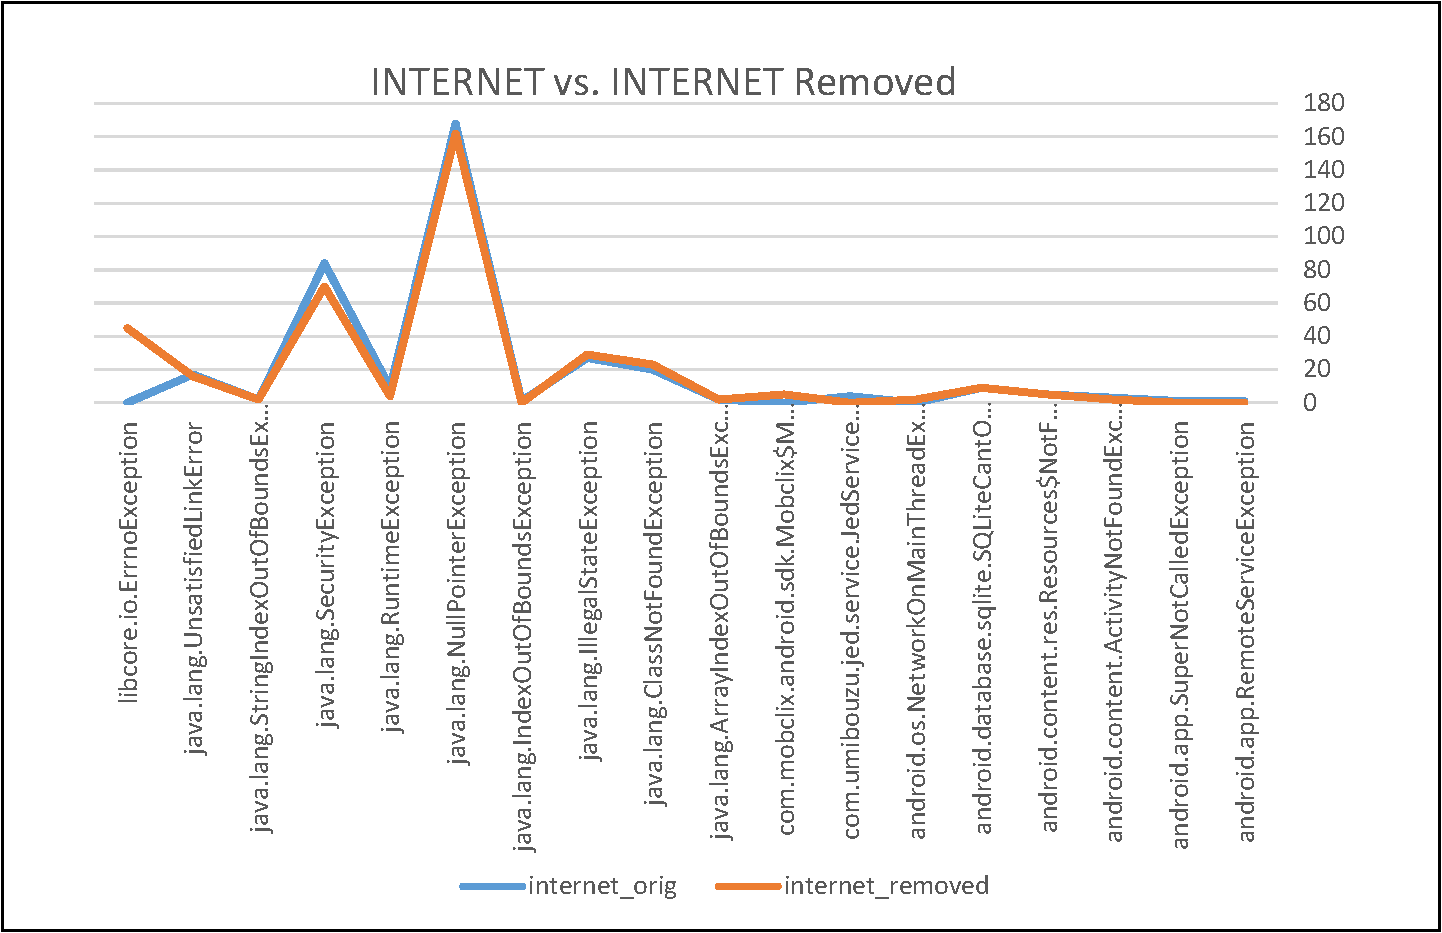
\includegraphics[width=8cm]{internet}\label{fig:internet}}
\hfill
\caption{Admob displays a message when the \texttt{INTERNET} permission is removedd~\ref{fig:removing} and Distribution of Exceptions with \texttt{INTERNET} permission~\ref{fig:internet}.}
\end{figure}
%\FloatBarrier


Since a significant number of applications were requesting the \texttt{INTERNET} permission for advertising purposes, a copy of a popular third-party Android web browser was attained for testing.  When executed with the \texttt{INTERNET} permission removed, the application terminated with a \texttt{SecurityException} related the applications request for DNS information. Upon further investigation, it was determined that the application calls the \texttt{java.net} functions directly, causing a \texttt{SecurityException} to be generated and the standard crash screen to be displayed (see Figure~\ref{fig:crash}).


%\FloatBarrier
\begin{figure}[h!]
\centerline{\resizebox{0.3\linewidth}{!}{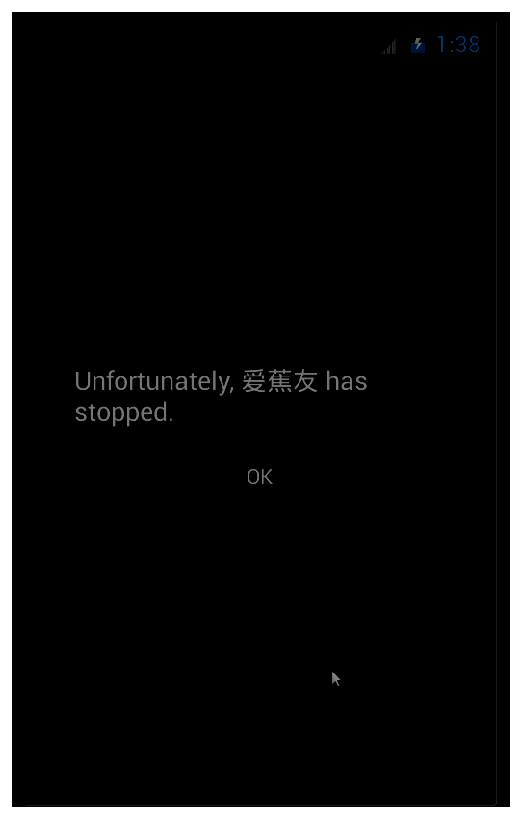
\includegraphics{figure3}}}
\caption{App crashes due to \texttt{SecurityException} when the \texttt{INTERNET} permission is removed.}
\label{fig:crash}
\end{figure}
%\FloatBarrier


\paragraph{{\bfseries \ttfamily CAMERA} and {\bfseries \ttfamily RECORD\_AUDIO}}
In the case of \texttt{CAMERA} and \texttt{RECORD\_AUDIO}, both functionalities have a service that proxies application requests.  If the relevant permissions are removed, they behave as if no camera or microphone is present.  Therefore, no \texttt{SecurityExceptions} were observed when these permissions were removed and the exception behavior of the applications showed no significant change (see Figure~\ref{fig:camera} and~\ref{fig:audio}).
%\FloatBarrier
\begin{figure}[h!]
\hfill
\subfigure[]{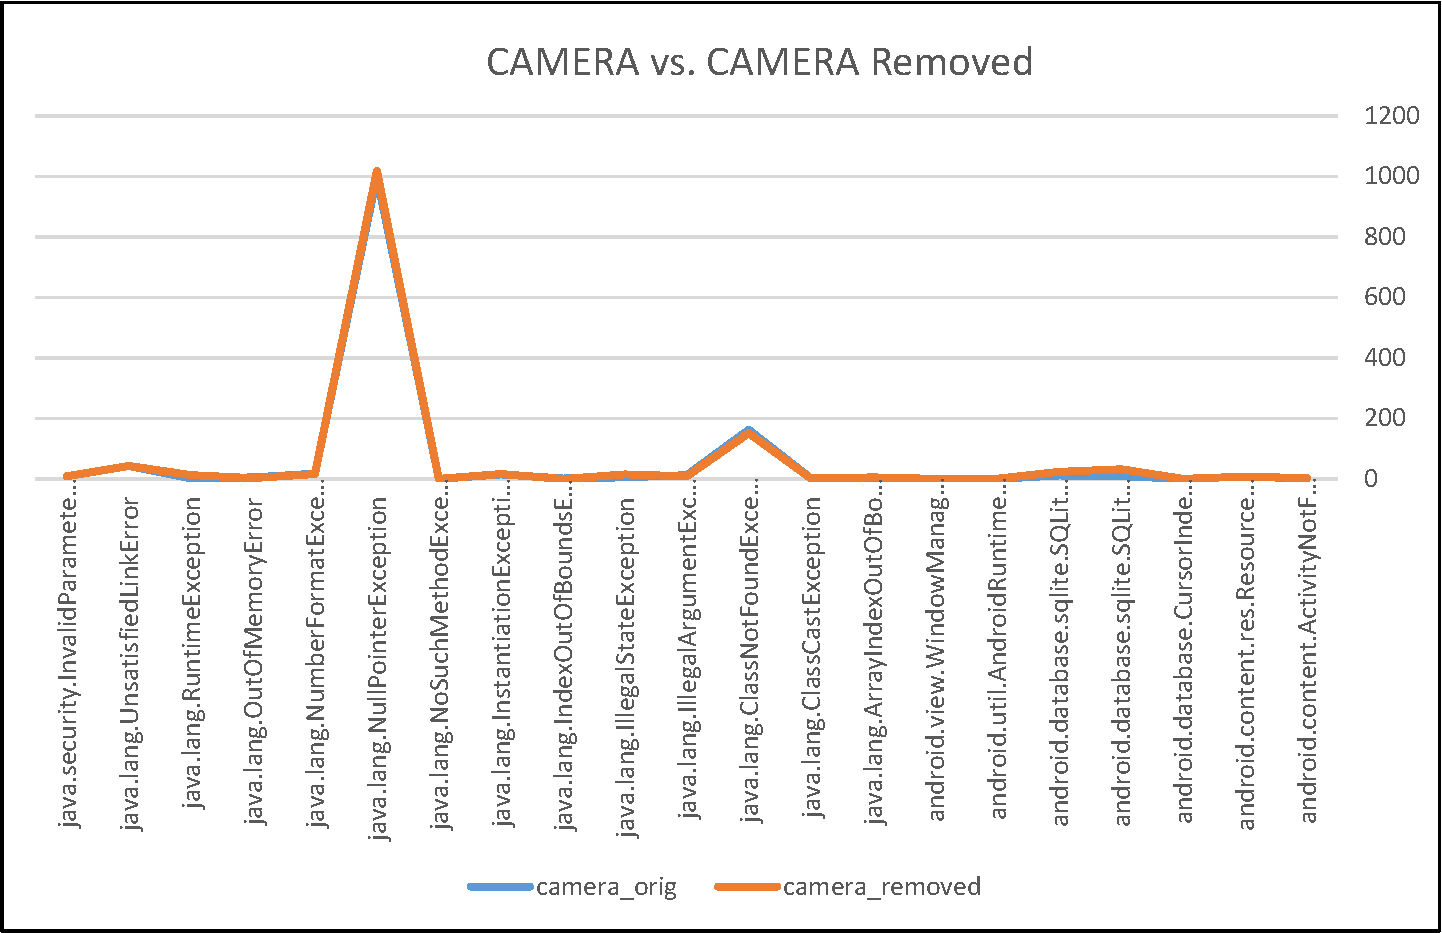
\includegraphics[width=8cm]{camera}\label{fig:camera}}
\hfill
\subfigure[]{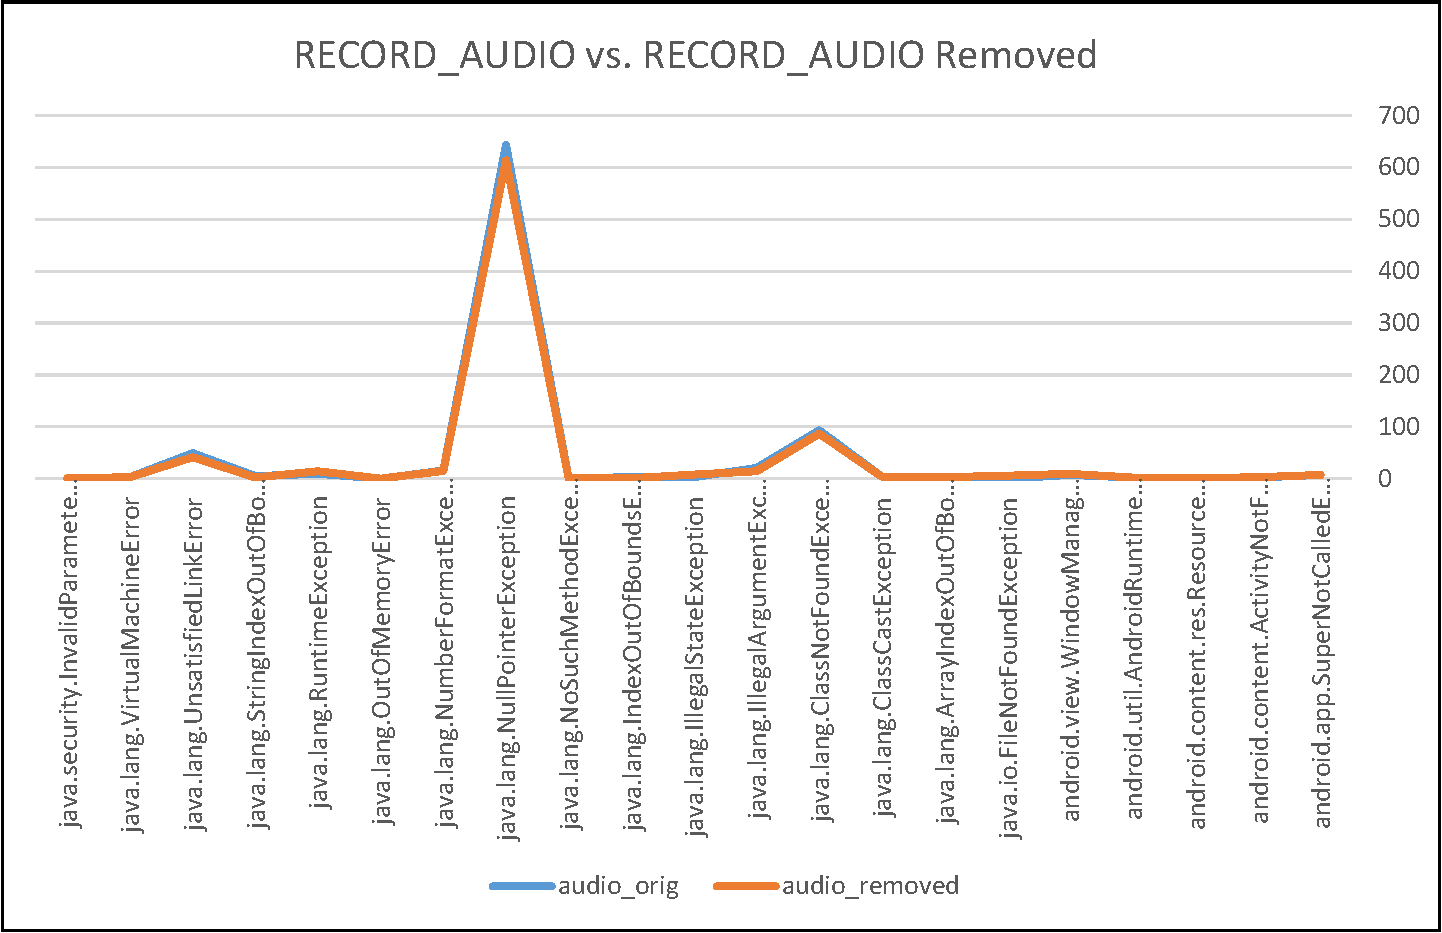
\includegraphics[width=8cm]{audio}\label{fig:audio}}
\hfill
\caption{Distribution of Exceptions for \texttt{CAMERA}~\ref{fig:camera} and \texttt{RECORD\_AUDIO}~\ref{fig:audio} permissions}
\end{figure}
%\FloatBarrier

\paragraph{{\bfseries \ttfamily READ\_CONTACTS} and {\bfseries \ttfamily READ\_CALENDAR}}
Manual investigation determined that, when removing \texttt{READ\_CONTACTS}, a \texttt{SecurityException} was only being recieved in cases where the API call to read the contacts was actually occurring. While the presence of some other helper library that catches exceptions cannot be completely ruled out, in every case that was manually examined, the \texttt{SecurityException} was only occurring when the automated testing specifically activated a UI element or activity's startup code that made a request to the Provider URI, \texttt{content://com.android.contacts/}. 

The removal of \texttt{READ\_CALENDAR} results in similar behavior. Apps attempting to access the Provider URI, \texttt{content://com.android.calendar/}, generated security exceptions in all cases that were examined.  When looking at the exception distribution plots for \texttt{READ\_CALENDAR} and \texttt{READ\_CONTACTS}, they both show the expected difference when their respective permissions were removed.  In the case of \texttt{READ\_CONTACTS}, however, there is an additional difference due to \texttt{com.scoreloop.client.android.ui.StandardScoreloopManager\$VerifyException}.  This error is due to an applications use of ScoreLoop, a cross-platform gaming SDK.  The SDK requires the \texttt{READ\_CONTACTS} permission and has its own exception handler written for when it is not declared in the manifest.

%\FloatBarrier
\begin{figure}[h!]
\hfill
\subfigure[]{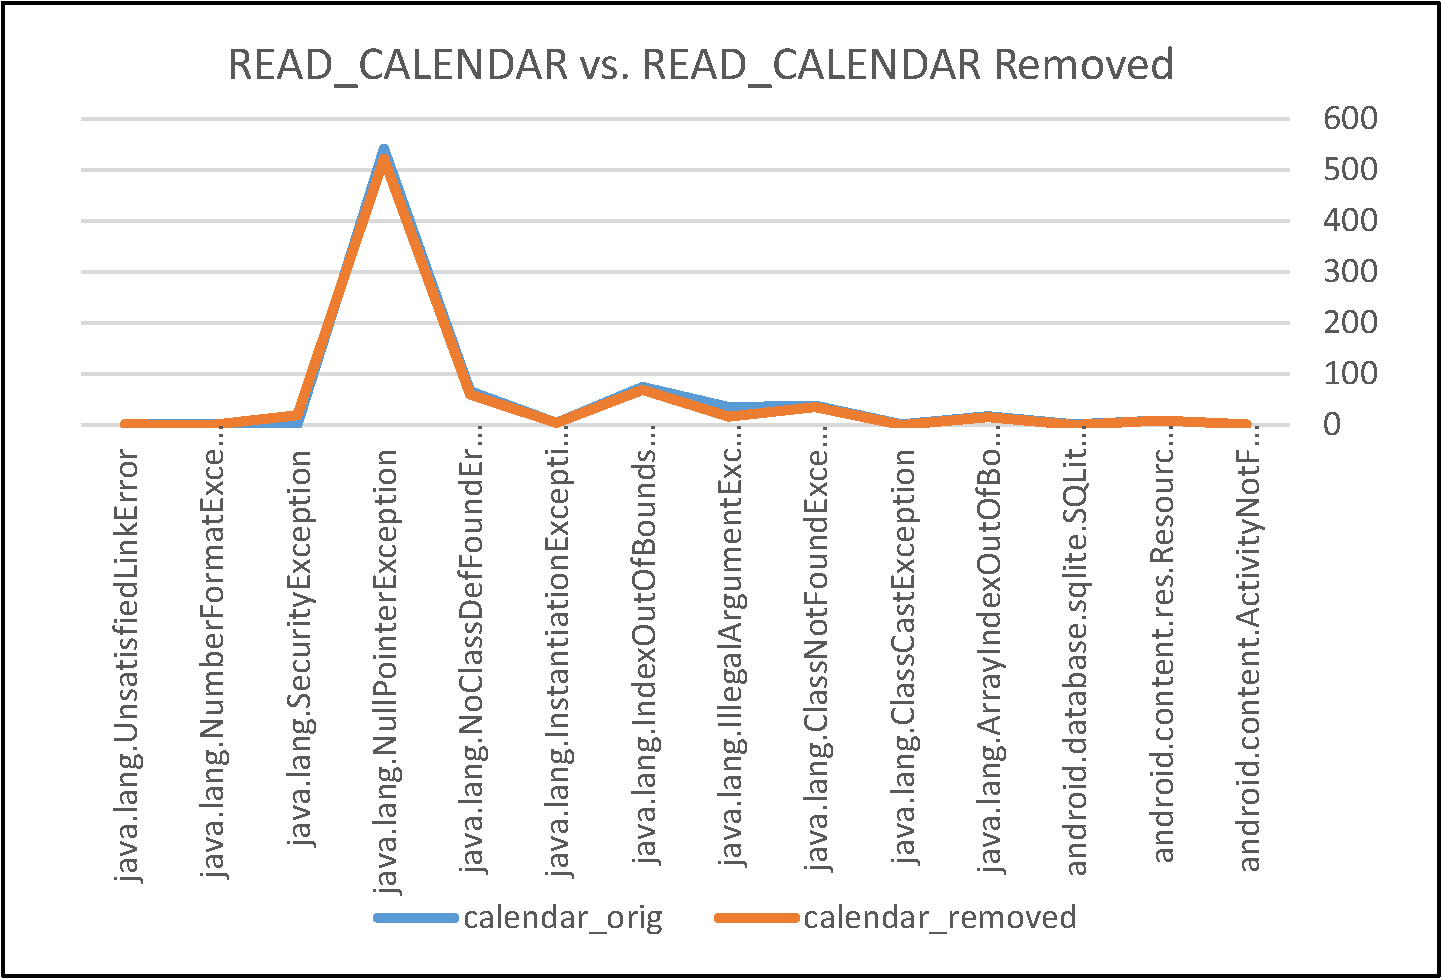
\includegraphics[width=8cm]{calendar}\label{fig:calendar}}
\hfill
\subfigure[]{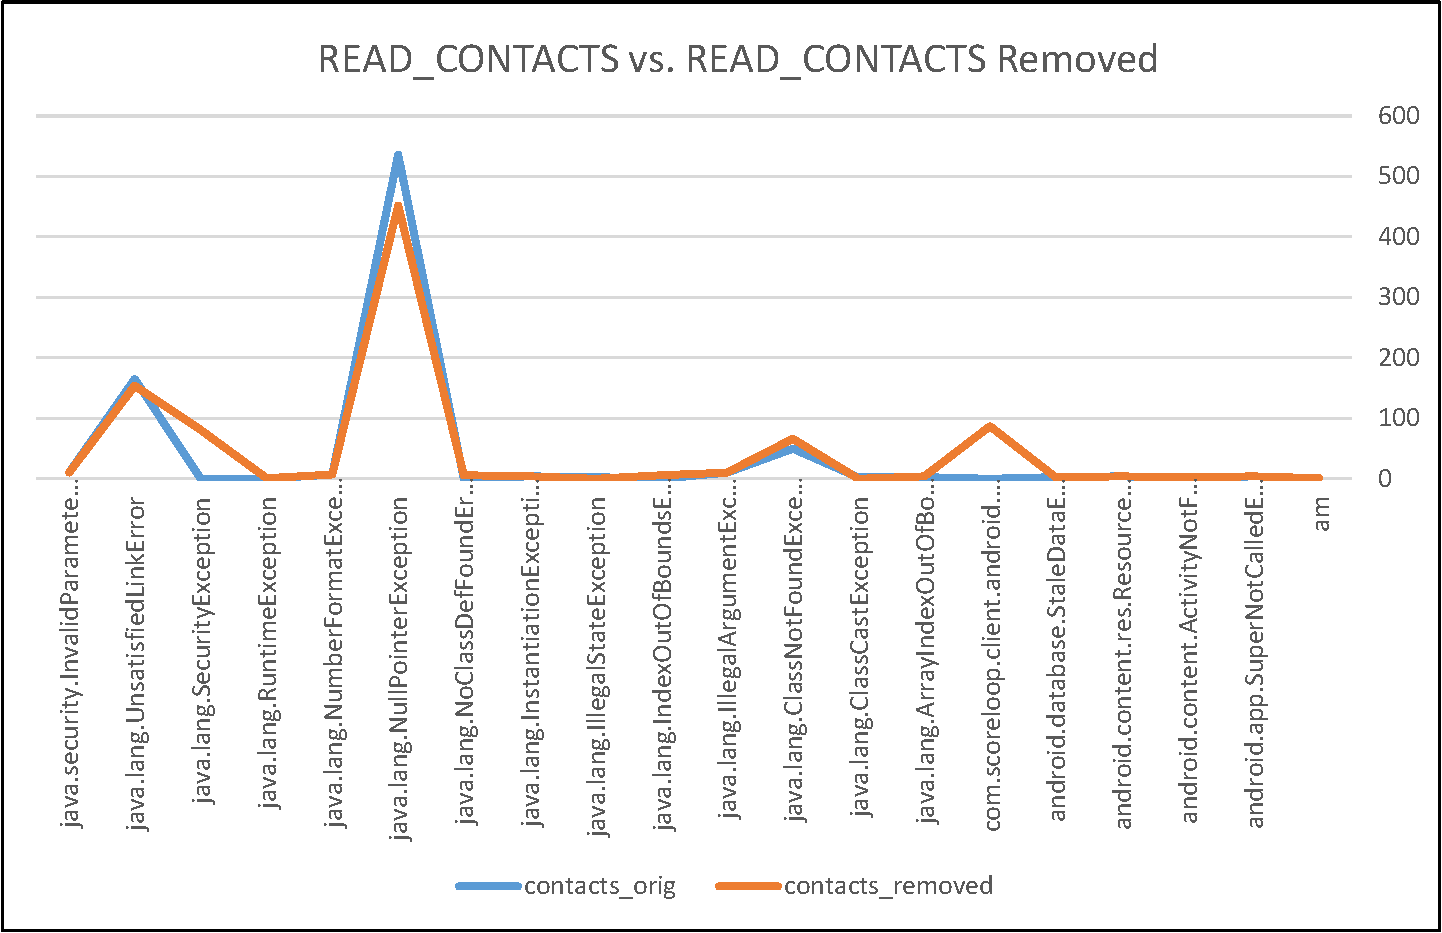
\includegraphics[width=8cm]{contacts}\label{fig:contacts}}
\hfill
\caption{Distribution of Exceptions for \texttt{READ\_CALENDAR}~\ref{fig:calendar} and \texttt{READ\_CONTACTS}~\ref{fig:contacts} permissions}
\end{figure}
%\FloatBarrier

\paragraph{\bfseries \ttfamily WRITE\_SMS}
The \texttt{WRITE\_SMS} permission also uses a Provider URI, \texttt{content://mms-sms/}; however, no \texttt{SecurityExceptions} resulting from permission removal were observed.  The one that was observed in both test cases was a result of the missing permission, \texttt{WRITE\_APN\_SETTINGS}, that was discussed earlier.  The lack of \texttt{SecurityExceptions} is likely due to the relative depth of writes to this URI within the application, which makes it more difficult to trigger.  Any unauthorized Provider URI access produces the standard crash screen (Figure~\ref{fig:crash}).  As expected, with no \texttt{SecurityExceptions} triggered, there was not significant difference in the distribution of errors when the permission of interest was removed. 

%\FloatBarrier
\begin{figure}[h!]
\hfill
%\subfigure[\texttt{WRITE\_SMS} permission]{\includegraphics[width=8cm]{sms-crop}}
\subfigure[]{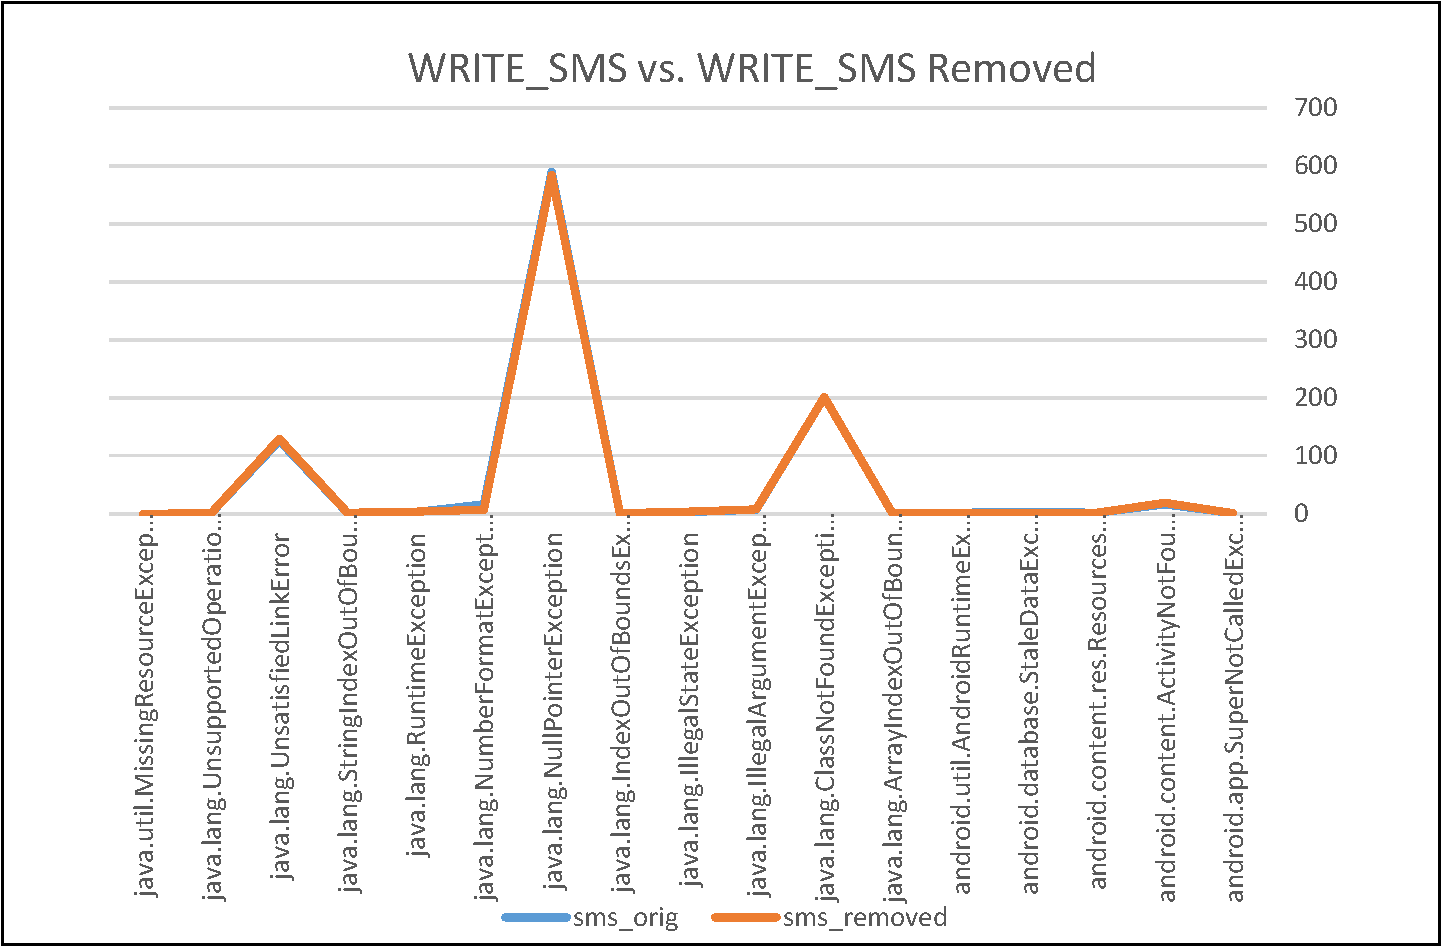
\includegraphics[width=8cm]{sms}\label{fig:sms}}
\hfill
%\subfigure[\texttt{ACCESS\_FINE\_LOCATION} permission]{\includegraphics[width=8cm]{location-crop}}
\subfigure[]{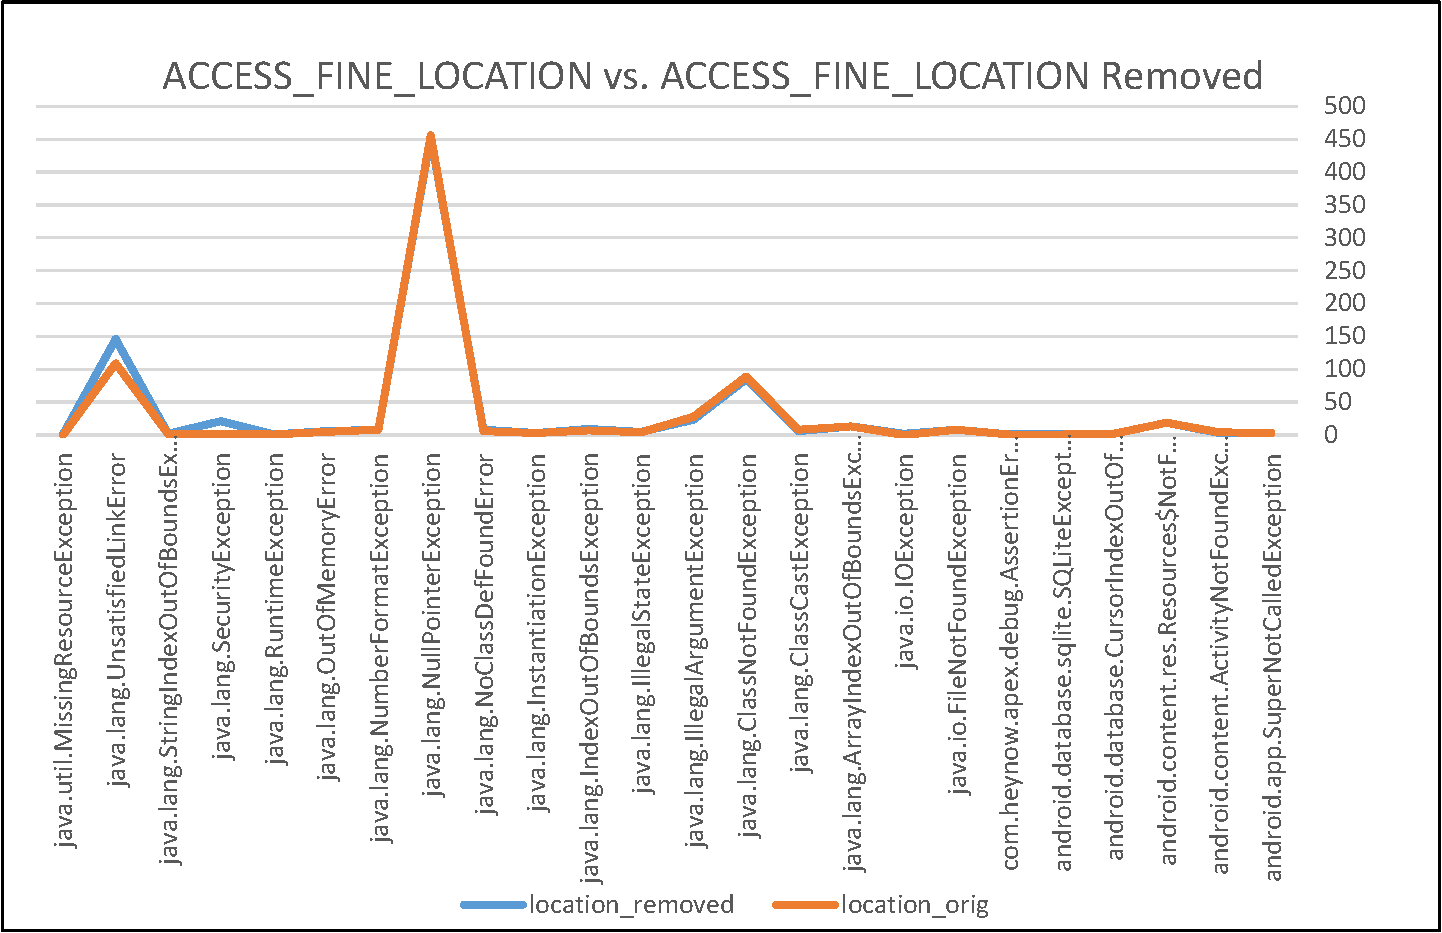
\includegraphics[width=8cm]{location}\label{fig:location}}
\hfill
\caption{Distribution of Exceptions for \texttt{WRITE\_SMS}~\ref{fig:sms} and \texttt{ACCESS\_FINE\_LOCATION}~\ref{fig:location} permissions.}
\end{figure}
%\FloatBarrier

\paragraph{\bfseries \ttfamily ACCESS\_FINE\_LOCATION}
The fine-grained location permission, \texttt{ACCESS\_FINE\_LOCATION}, is a special case. It is one of a few permissions in Android that is a nested permission. Many API calls will operate in the presence of either fine or coarse location permissions but prefer fine; if fine is removed they will fall back to coarse grain location. This results in few \texttt{SecurityExceptions} (\textasciitilde12\%), since they will only occur in cases where the GPS hardware is explicitly being used.  Comparing the distribution of exceptions, the removal of the \texttt{ACCESS\_FINE\_LOCATION} permission does not appear to have any significant impact on exceptions outside of causing \texttt{SecurityExceptions}.
